\documentclass{article}
\usepackage[margin=1.2in]{geometry}
\usepackage{datetime}
\usepackage{hyperref}      %for \url macro
\usepackage{microtype}     %attempt to fix issue with justification protrusion (in references)
\usepackage{amssymb}       % for formatting less/greater than symbols
\usepackage{amsmath}
\usepackage{enumitem}      %for changing spacing in bulleted lists
\usepackage{subfigure}        %for subfigures


\renewcommand{\arraystretch}{1.25}

\usepackage[gobble=auto, runall=true]{pythontex}
\usepackage{float} %for forcing position of images

\usepackage{graphicx}
\graphicspath{ {../images/} }
\usepackage[export]{adjustbox}
\usepackage[justification=centering]{caption}

\usepackage{listings}   %for typesetting code
\usepackage{color}
\definecolor{codegreen}{rgb}{0,0.6,0}
\definecolor{codegray}{rgb}{0.5,0.5,0.5}
\definecolor{codepurple}{rgb}{0.58,0,0.82}
\definecolor{backcolour}{rgb}{0.95,0.95,0.92}
\lstdefinestyle{mystyle}{
    backgroundcolor=\color{backcolour},
    commentstyle=\color{codegreen},
    keywordstyle=\color{codepurple},
    numberstyle=\tiny\color{codegray},
    stringstyle=\color{codepurple},
    basicstyle=\footnotesize,
    breakatwhitespace=false,
    breaklines=true,
    captionpos=b,
    keepspaces=true,
    %numbers=left,
    numbersep=5pt,
    showspaces=false,
    showstringspaces=false,
    showtabs=false,
    tabsize=2
}
\lstset{style=mystyle}

\frenchspacing                   %removes extra spacing after a period at the end of a sentence.
\newdateformat{daymonthyear}{\THEDAY\ \monthname\ \THEYEAR}

\title{CSC411 Machine Learning \\ Project 3: Fake News}
\author{ Ariel Kelman \\ Student No: 1000561368
         \\ \\
         Gideon Blinick \\ Student No: 999763000 }
\daymonthyear



\begin{document}
   \maketitle{}


   \section{Dataset Description}

   Both datasets (real and fake) contain headlines about U.S. President Donald Trump.
   From the headlines, it is possible to determine with significant accuracy
   the probability that a given headline is fake or real based simply on the presence or
   absence of particular words in the headline. For example, after performing some preliminary
   analyses on the headlines, we discovered that the following 3 words might be of particular use.
   \begin{enumerate}
      \item The word ``donald'' appears 42.05\% of the time in real headlines while appearing in only
            17.55\% of fake headlines. This 24.5\% difference was by far the largest of any word.
      \item The word ``the'' appears 27.9\% of the time in fake headlines while appearing in only
            7.9\% of real headlines, for a difference of 20.02\%.
      \item The word ``trumps'' appears 11.1\% of the time in real headlines while appearing in
            only 0.3\% of fake headlines, for a difference of 10.8\%.
   \end{enumerate}

   The data was split into a training, validation, and testing set for analysis in the remainder
   of the report.


   \subsection{Results \& Report Reproducibility}
   All results and plots can be generated using the code in \texttt{fake.py}.
   All code is python 3, run with Anaconda 3.6.3.
   Running the code will save all generated images in the \texttt{resources} folder,
   where they are used by \LaTeX. Note that some of the sections require the code for
   other sections (in the same file) to be run first.
   To reproduce the report, simply run it through \LaTeX. This will pull the most recently
   generated figures from the \texttt{resources} folder.


   \section{Naive Bayes Implementation}
   The Naive Bayes algorithm was implemented in three primary functions.
   In the first function \texttt{traing\_part()} we use the training set to achieve estimates for $p(real)$,
   $p(fake)$, $p(word\ |\ real)$ and $p(word\ |\ fake)$. We estimated $ p(word\ |\ real)$ and $p(word\ |\ fake)$ by counting
   the number of headlines in the training set where the word appears and the headline is real (or fake), adding a
   factor of $ m \cdot p$, and divided this result by the size of the training set plus $m$. We also included
   words that were not found in the training set (but found in validation or testing) and set their
   values to $ \frac {m \cdot p}{count(headlines) + m}$, i.e. the value they would have from a count of zero in
   the training set. This function returns the values of $p(real)$ and $p(fake)$
   and dictionaries with the remaining information.

   In the next stage, we created a function \texttt{evaluate()} which uses the outputs of the first
   function -  $p(real)$, $p(fake)$, $p(word\ |\ real)$, $p(word\ |\ fake)$ - to
   compute $p(headline\ |\ real)$ and $p(headline\ |\ fake)$ for a given set of headlines, and in turn uses
   those to compute $p(real\ |\ headline)$ and $p(fake\ |\ headline)$ for the set of headlines, which is
   the function output. To avoid ``underflow'' caused by the multiplication of many small numbers (the
   probabilities for each word are quite low, as most words appear in a small fraction of headlines),
   we utlize the fact that
      \begin{equation*}
         a_1 \cdot a_2\ ...\ \cdot a_i =  e^{ln(a_1) + ln(a_2) + ... + ln(a_i)}
      \end{equation*}
   in order to compute $p(headline\ |\ real)$ as the product of $p(word\ |\ real)$ for all words.

   The final step in the implementation the accuracy is checked (using the function \texttt{check\_accuracy()}
   with a threshold of 0.5), and the parameters $m$ and $p$ were tuned to produce the best accuracy on
   the validation set. This was done via a simple search (see the function \texttt{optimize\_mp()}).
   We began with a value of $m = 2 \cdot 5833 $ and $p = \frac {1}{2 \cdot 5833}$ and optimized from there.
   This was chosen as our starting point as is 1 example per class per word, which is intuitively what adding in
   the $m$ and $p$ factors are trying to do - avoiding the issue of too few counts.
   Some of the values tested are shown in the following table.
   %We then chose 4 different values of m and p and tested how they perform on our validation set, via a function
   %called "optimize\_mp()".

      \begin{table}[h]
         \centering
         \renewcommand{\arraystretch}{1.5}

         \begin{tabular}{ c|c }
            \hline
            $m$ & accuracy \\
            \hline \hline
            $1 \cdot 5833$ & 90.4\% \\
            $2 \cdot 5833$ &  90.4\% \\
            $3 \cdot 5833$ &  90.4\%  \\
            $4 \cdot 5833$ &  90.4\%  \\
            \hline
         \end{tabular}

         \caption{ Some tested values for optimizing Naive Bayes, and the corresponding accuracy on the
               validation set.}
      \end{table}


   We discovered that all our choices for $m$ and $p$ lead to the same accuracy of 90.4\%, so we decided to stay
   with our initial values for $m$ and $p$ of 2 and 5833, respectively. These values gave an accuracy of 92.3\% on
   the training set, and on the testing set we achieved an accuracy of 92.2\%.


   \section{Predictive Factors for Naive Bayes}
   \subsection{Predictive Words}
   The following bullet points present the top 10 words whose presence or absence most strongly indicate that a headline is real/fake
   based on the naive bayes analysis above. Note that for some classes,
   such as $p(real \ |\ word)$, there were many other words that could have been in the list provided, as the probabilites were quite high
   (many words appeared \textit{only} in the fake or real training set).
   \begin{enumerate}
      \item Maximize $p(real \ |\ word)$:
              %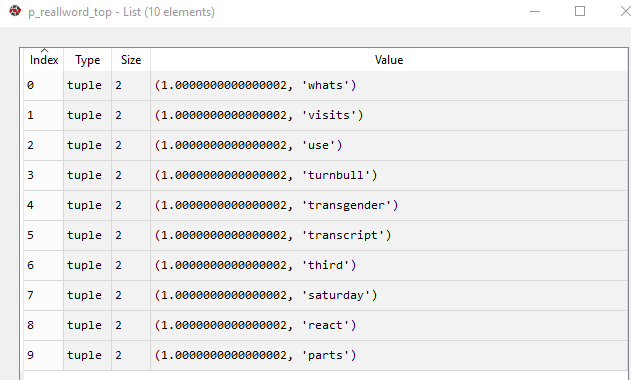
\includegraphics[width=4in]{resources/part3/p(realword)}
   	          ``xi'', ``wrap", ``whats", ``west", ``turnbull", ``troops", ``travel", ``tourism", ``tillerson", ``third"
      \item Maximize $p(real \ |\ \neg word)$:
             % 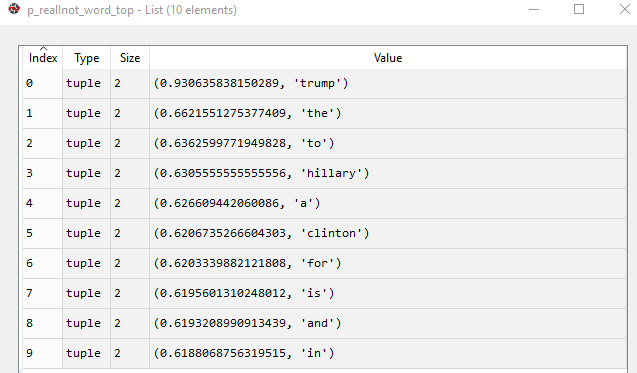
\includegraphics[width=4in]{resources/part3/p(realnotword)}
   	         ``trump", ``the", ``to", ``hillary", ``a", ``is", ``and", ``for", ``in", ``of"
      \item Maximize $p(fake \ |\ word)$:
             % 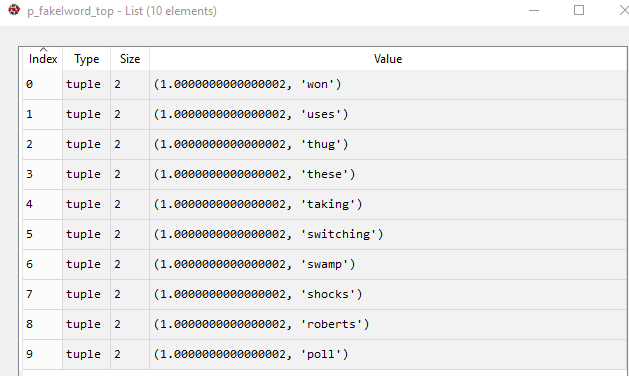
\includegraphics[width=4in]{resources/part3/p(fakeword)}
   	         ``thug", ``these", ``surprise", ``supression", ``story", ``steal", ``start", ``soros", ``save", ``protestor"
      \item Maximize $p(fake \ |\ \neg word)$:
             % 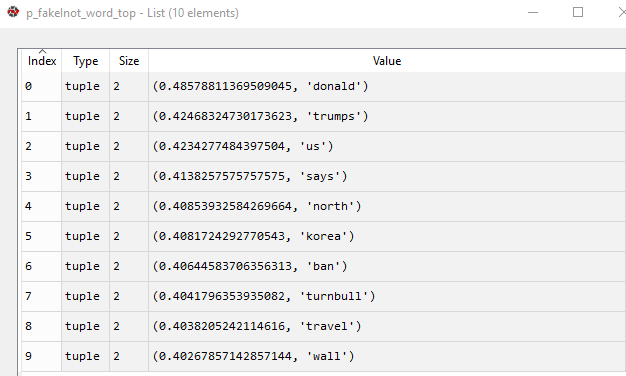
\includegraphics[width=4in]{resources/part3/p(fakenotword)}
   	         ``donald", ``trumps", ``us", ``north", ``says", ``korea", ``ban", ``turnbull", ``travel", ``wall"
   \end{enumerate}

   These values were obtained by applying Bayes rule. More specifically, we calculated $p(real \ |\ word)$ by
   $ \frac {p(word \ |\ real) \cdot p(real)}{p(word)}$. $p(word \ |\ real)$ can be obtained for every word by taking
   the number of headlines with a given word in the training set that are also real and dividing it by the
   total number of headlines that are real in the training set. $p(real)$ is the number of headlines in the
   training set that are real divided by the total number of headlines in the training set. Finally, $p(word)$ is
   the number of headlines in the training set with the word divided by the number of headlines in the training set.
   All these are easily obtained.

   To obtain $p(real \ |\ not\_word)$, we use $ \frac {p(not\_word \ |\ real) \cdot p(real)}{p(not\_word)}$. p(real)
   is the same from the previous step, $p(not\_word \ |\ real)$ is 1 - $p(real \ |\ word)$, and $p(not\_word)$ is the
   number of headlines without a word in the training  set divided by the total number of headlines.
   The calculcations for $p(real \ |\ word)$ and $p(real \ |\ not\_word)$ proceed in an equivalent way with an
   appropriate substitution of "fake" for any mention of "real".

   What is observable from looking at the numbers associated with these results is that the presence of certain
   words has far greater predictive ability than the absence of any given word. This is reasonable,
   as the headlines are quite short (relative to the number of total words), so most ``vectors'' representing
   a headline are sparse, and that sparsity is the same for both real and fake headlines.
   It is particularly intersting to note, however, how strongly the absence of stop words indicates that a
   headline is real.

   \subsection{Without Stop Words}
   If we ignore stop words (obtained from \texttt{sklearn} as suggested), the following lists show the top words
   whose presence indicate that a word is real/fake. Only 1 stop word was included in the lists above (looking at
   words whose \textit{presence} matters) however, so these words are almost identical to those above.
   \begin{enumerate}
      \item Maximize $p(real \ |\ word)$:
         ``xi", ``wrap", ``whats", ``west", ``turnbull", ``troops", ``travel", ``tourism", ``tillerson", ``third'' %``sessions"
      \item Maximize $p(fake \ |\ word)$:
         ``thug", ``surprise", ``supression", ``story", ``steal", ``start", ``soros", ``save", ``protestor", ``msnbc"
   \end{enumerate}

   \subsection{Stop Words}
   %Removing stopwords might make sense because stop words just might by change have a large discrepency in the
   %training data that has no real predictive ability, and therefore cause the model to overfit. It might make
   %sense to keep stopwords because they may in fact have predictive ability.
   When interpreting the model, stop words do not seem like the type of words that would be important, as they
   do not reflect ideas related to the classification of a headline as real or fake, and it is perhaps more
   likely that any patterns found in stop words are due to the division of the training and other sets.
   However, it is reasonable to suppose that real news outlets do use stop words differently than fake news
   outlets, in which case, they are important to building and interpreting the model. Analysis including stop
   words may even provide a way to learn about how stop words are used by different media types.


   \section{Logistic Regression}
   Code from project 2 was modified to run simple logistic regression to predict whether a headline is real
   or fake. For each headline, a sparse vector was created, with $1$'s in each position that represents a word
   that's present in the given headline (the representation of this vector is discussed again in section 5).
   The outputs were passed through the softmax function to produce results that can be interpreted probabalistically.

   A regularization term was added directly to the gradient function that penalizes the L1 norm of the
   $\theta$'s (the parameters of the regression).
   To determine the best values for the learning rate and the weighting of the L1 regularization term (parameterized
   by $\gamma$), a simple grid search was preformed (primarily focussed on varying $\gamma$), using the results on
   the validation set to determine the best hyperparameters. The learning curves for many of these tests can be
   found in the \texttt{resources/part4} directory.

   The following learning curves shows the results for the hyperparameter settings $\gamma = 1$ with a learning
   rate of $10^{-3}$, though the results did not vary much with changes to $\gamma$. It is curious, but likely due
   to random sampling, that the testing set consistently preforms better than the validation set.
   \begin{figure}[h] \centering
      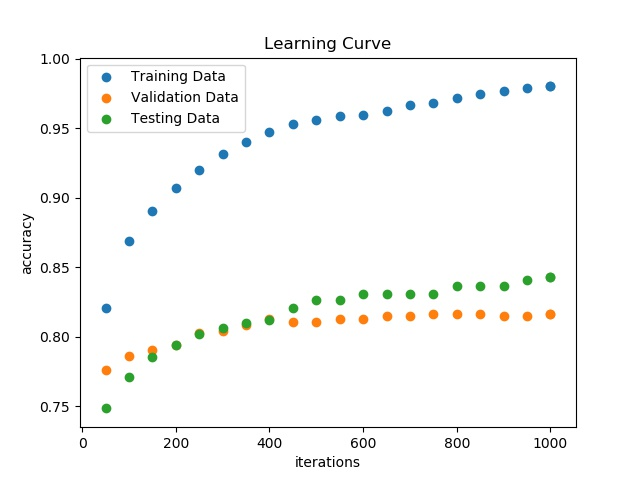
\includegraphics[width=4in]{resources/part4}
      \caption{ Learning curve for the logistic regression with a learning rate of $10^{-3}$ and
            $\gamma = 1$.}
   \end{figure}

   These parameters gave a final training accuracy of 98\%, validation accuracy of 81.7\%, and testing
   accuracy of 84.3\% (likely due to the random division of data among the sets) after 1000 iterations.



   \section{Logistic Regression vs. Naive Bayes}
   When forming a prediction on a headline, both Naive Bayes and Logistic Regression effectively compute
   \begin{equation*}
      \theta^T I = \theta_0 + \theta_1 I_1 + \theta_2 I_2 + ... + \theta_k I_k > thr
   \end{equation*}
   where $thr$ is a given threshold value; in this project $thr = 0.5$. In both cases, the $\theta$'s represent
   the paremeters that define the prediction model, while the $I$'s are a function of the input for which a
   prediction is produced.

   For logistic regression, each $I = I(x)$ for a headline is simply a vector of $0$'s and $1$'s, where each
   position in the vector represents a word that was included in the training set. A $1$ indicates that the
   word is found in the headline, while a $0$ indicates that one was not. As the headlines are relatively short
   in comparison to the total number of words, this vector is very sparse. The $\theta$'s represent how important
   a feature (the presence of a particular word) is to the final prediction ($\theta_0$ is a bias that can
   account for the priors on real vs. fake headlines).

   For naive bayes, consider the log-odds of a headline belonging to a particular class (real or fake). The
   classifier computes the log odds of each word appearing in a headline given each class
   ($ln \big[ \frac{p(word | c)}{p(word | ~c)} \big]$; the bias is simply $ln \big[ \frac{p(c)}{p(~c)}\big]$).
   These log-odds are represented by $\theta$, each $\theta_i$ is the log-odds of the corresponding word.
   As before, $I_i$ is 1 when the word is in the headline and 0 otherwise.



   \section{Analysis of Logistic Regression}
   Table \ref{part6table} shows the words that had the most impact on the classification of a headline
   as real or fake via logistic regression. Some, but not all, of these words appeared as significant
   in the naive bayes implementation, such as ``trmups,'' ``us,'' ``turnbull,'' etc. Note that the (absence
   of) stop words was significant for naive bayes, but do not seem to play a significant role in
   the regression classification.

   \begin{table}[h]
      \centering
      \renewcommand{\arraystretch}{1.5}

      \begin{tabular}{ p{7em}|l || p{7em}|l }
         \hline
         word     &     $\theta_i$   & word & $\theta_i$   \\
         \hline \hline
         trumps      &     -5.2        &  breaking    & 2.63    \\
         us          &     -2.7        &  america     & 2.45    \\
         says        &     -1.87       &  hillary     & 2.37    \\
         comey       &     -1.79       &  just        & 2.28    \\
         turnbull    &     -1.76       &  u           & 2.14    \\
         ban         &     -1.71       &  black       & 2.06    \\
         donald      &     -1.68       &  victory     & 2.05    \\
         meeting     &     -1.68       &  are         & 1.99    \\
         korea       &     -1.68       &  watch       & 1.85    \\
         flynn       &     -1.67       &  an          & 1.81    \\
         \hline
      \end{tabular}

      \caption{ The words (and corresponding $\theta_i$'s) that have the most impact
               on classification via logistic regression.}
      \label{part6table}
   \end{table}


   \subsection{Ignoring Stop Words}
   If we eliminate the stop words in the above table, the list in table \ref{part6table2} shows the highest (in magnitude)
   values in $theta$ and the corresponding words. (Note that the logistic regression itself still uses stop
   words, they are simply ignored in this analysis). Once again, some of these words correspond to those
   in part 3 (when stop words were ignored), though quite a few are new (e.g. ``breaking'').

   \begin{table}[h]
      \centering
      \renewcommand{\arraystretch}{1.5}

      \begin{tabular}{ p{7em}|l || p{7em}|l }
         \hline
         word     &     $\theta_i$   & word & $\theta_i$   \\
         \hline \hline
         trumps      &     -5.2        &  breaking    & 2.63    \\
         says        &     -1.87       &  america     & 2.45    \\
         comey       &     -1.79       &  hillary     & 2.37    \\
         turnbull    &     -1.76       &  just        & 2.28    \\
         ban         &     -1.71       &  u           & 2.14    \\
         donald      &     -1.68       &  black       & 2.06    \\
         meeting     &     -1.68       &  victory     & 2.05    \\
         korea       &     -1.68       &  watch       & 1.85    \\
         flynn       &     -1.67       &  putin       & 1.7     \\
         trump       &     -1.66       &  elect       & 1.67    \\
         \hline
      \end{tabular}

      \caption{ The words (and corresponding $\theta_i$'s) that have the most impact
               on classification via logistic regression, ignoring stop words.}
      \label{part6table2}
   \end{table}



   \subsection{Analyzing Parameters}
   In the analysis of the logistic regression preformed above, the magnitude of the regression parameters
   were taken to signify the importance of the associated features (i.e. the presence of a particular word)
   to classification. In general this may be problematic, as different features may have different
   magnitudes (to take an example discussed in lecture, house prices and number of rooms may be features that
   are important to predicting selling price, but house prices are numerically much larger than the number of
   rooms in a house), in which case the magnitude of the parameters will differ from the effect they have on
   prediction.
   However, in the logistic regression for classifying headlines, all features have equal magnitude (when
   they are present). Therefore, no bias is introduced by these features that impacts on the classification
   other than the $\theta$'s - so the magnitude of $\theta_i$ is indicative of the importance of the
   corresponding word.



   \section{Decision Tree}
   \subsection{Classification}
   Using the \texttt{sklearn} implementation of decision trees, we trained several decision trees
   to differentiate between the fake and real headlines. After some experimentation with the many parameters
   in the \texttt{sklearn DecisionTreeClassifier} (particularly with the maximum number of features used
   when looking for the best split), the default parameters gave the best results. As a split condition,
   maximum entropy was used rather than gini impurity, though similar results were obtained for both.
   Many of the settings served as ways to limit the size of the decision tree, so this result is not unexpected.

   Decision trees with a maximum depth of $\{ 2, 3, 5, 10, 15, 20, 35, 50, 75, 100, None \}$ were built, and
   the results on the training, validation, and testing sets are shown figure \ref{part7a} below. The final point,
   not plotted, with no limit on the maximum depth, gave an accuracy of $1, 0.76 0.76$ on the training,
   validation, and testing sets respectively.
      \begin{figure}[h] \centering
         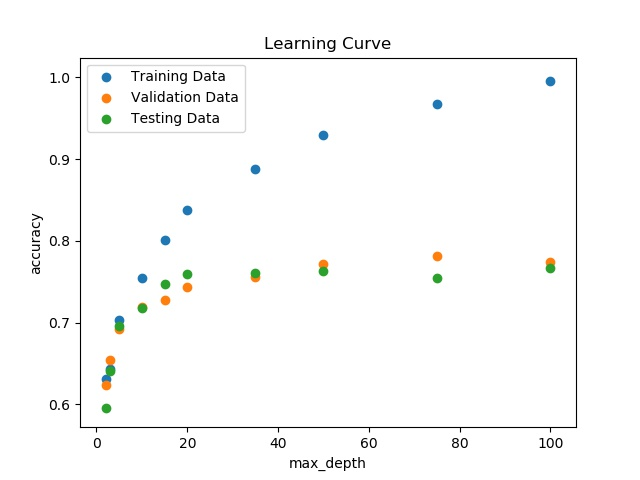
\includegraphics[width=4in]{resources/part7/part7a_splitCondition=entropy_maxFeatures=None_stopWords=True}

         \caption{Plot showing the preformance of \texttt{sklearn} decision trees with
            varying depth. The split condition was maximum entropy, there was no limit on the maximum
            number of features for a split, and stop words were included.}
         \label{part7a}
      \end{figure}
   As can be seen from the figure, the larger the depth of the decision tree, the greater accuracy achieved on
   the testing set. However, improvement is small on the validation and testing sets after a depth of
   $~20$. Without any other constraints (such as a minimum number of samples to split a node), a decision tree
   can reach perfect accuracy on the training set, as demonstrated above. Predictably, this leads to
   much greater preformance on the training set than on the validation and testing sets (though there is no
   \textit{decrease} in preformance on the latter sets); showing the importance of using a validation and testing
   set to measure preformance.

   \subsection{Visualization}
   The following image shows the first few layers of the decision tree with depth $20$. It was generated by saving
   a text representation of the tree (as a \texttt{.dot} file), which was then visualized using the
   \texttt{webgraphviz} tool (available at \url{http://webgraphviz.com/}).
      \begin{figure}[h] \centering
         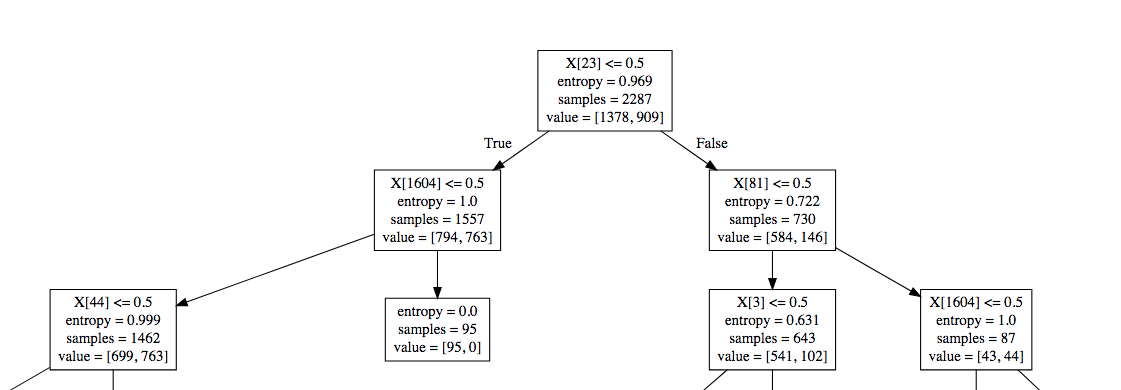
\includegraphics[width=4in]{resources/part7b}
         \caption{The top few layers of the decision tree (depth = 20).}
         \label{part7b}
      \end{figure}

   It is interesting to look at the words being split on in these layers; $X$ was a list of all words
   that appeared in either the fake or real datasets. These words are `donald' (23), `trumps' (1604; note the
   double appearance), `the' (81), `hillary' (44), and `trump' (3). These words are recognizable from earlier
   sections (parts 1, 3, and 6) as also playing a significant role in classification for the other classifiers.
   The exact same process of training was run
   ignoring stop words, but results were slightly worse; graphs similar to those mentioned above can be found
   in the \texttt{resources} directory (each filename indicates whether stop words were included, as well as info
   on the other non-default parameters). Note that because of the use of dictionaries (i.e. because
   \texttt{dict.keys()} does not keep track of order), running the code again may result in different indices
   for each of the above words.


   A visualization of the entire tree is saves as \texttt{part7b\_all.pdf}
   in the \texttt{resources} directory; the text represenations of many trees that were generated during
   training are saved in \texttt{resources/part7}.

   \subsection{Comparison of All 3 Classifiers}
   All three classifiers preform much better than random guessing, and quite well considering the
   difficulty of the task. Of the three classifiers, Naive Bayes had the best preformance (83.4\%, 83.7\%,
   and 84.7\% on the training, validation, and testing sets respectively), slightly beating the logistic
   regression classifier (98\%, 81.7\%, and 84.3\%). Though the difference is slight, it is notable that
   Naive Bayes achieves this accuracy despite making the extra assumption of conditional independence. It
   is also worth noting that Naive Bayes does not have significantly higher accuracy on the training set than
   on the validation or test sets.
   In last place is the decision tree mentioned above (depth 20, no limit on the maximum number of features
   used for splitting, and \textit{entropy} as the metric for the quality of a split), which gave an accuracy
   of 83.8\%, 73.7\%, and 75.7\% on the respective sets.




   \section{Information Theory}
   \subsection{Mutual Information on First Split}
   Using the result from part 7, the word that produced the best initial split was `donald'. The mutual information
   (a measure of `information gain') on that split (on the training data) can be calculated by
   \begin{equation*} \begin{split}
      I(Y, x)  &= H(x) - H(x, Y) = H(Y) - H(Y,x)
   \end{split} \end{equation*}
   where $I$ is the mutual information, $H(x)$ is the entropy of $x$, and $H(x, Y)$ is the entropy of $x$ conditional
   on $Y$.
   Plugging in the values shown in Figure \ref{part7b} gives
   \begin{equation*} \begin{split}
      I(Y, x)  &= H(Y) - H(Y,x) \\
               &= 0.969 - \bigg[ P_1 (1) + P_2 (0.722)  \bigg] \\
               &= 0.969 - \bigg[ \frac{1557}{2287} (1) + \frac{730}{2287} (0.722)  \bigg] \\
               &= 0.0557
   \end{split} \end{equation*}
   where $x = `donald'$ and $Y$ indicates whether a headline is real or fake.

   A function \texttt{mutual\_info()} was written to check this result, and to calculate the mutual
   information for other possible splits. The code for this function is shown below; it gave a result
   of 0.58 for $x = `donald'$.

      \begin{lstlisting}[language=Python]

         def mutual_info(word, y):
             count_word = 0 #number of headlines with word in training set
             lines_with_word = []
             lines_without_word = []
             for k in range(len(training_set)):
                 if word in training_set[k]:
                     count_word += 1
                     lines_with_word += [k]
                 else:
                     lines_without_word += [k]
             prob_word = count_word/len(training_set)

             y_with = np.array( [y[i] for i in lines_with_word] )
             y_without = np.array( [y[i] for i in lines_without_word] )

             prob_fake = np.count_nonzero(y)/len(y)
             H = prob_fake*np.log(prob_fake) + (1 - prob_fake)*np.log(1 - prob_fake) #entropy before split
             H = - H/np.log(2) #convert to base 2, and apply negative

             prob_fake_with = np.count_nonzero(y_with)/len(y_with)
             Hy = prob_fake_with*np.log(prob_fake_with) + (1 - prob_fake_with)*np.log(1 - prob_fake_with)
             Hy = - Hy/np.log(2) #entropy of headlines with word

             prob_fake_without = np.count_nonzero(y_without)/len(y_without)
             Hn = prob_fake_without*np.log(prob_fake_without) + (1 - prob_fake_without)*np.log(1 - prob_fake_without)
             Hn = - Hn/np.log(2)  #entropy of headlines without word

             I = H - (Hy*len(y_with) + Hn*len(y_without) )/len(y)
             return I
      \end{lstlisting}



   \subsection{Mutual Information on Later Split}
   The same procedure can be followed to compute the mutual information for a split on another word.
   Choosing a word randomly, gave a value of 0.0013 for the mutual information of a split of the training
   set on the word `ways'. As expected, this value is lower than the mutual information for a split on the
   word `donald' - that word was chosen as the first split precisely because it gave the most information
   about whether a headline was real or fake.



\end{document}
